\chapter{Results}
\label{c:results}

This chapter presents the main results in a logical succession, corresponding with the objectives defined in the \nameref{s:intro:need-for-transition} section. The development of the vision of a future sustainable mobility system is given in \autoref{s:results:ssp1-mob}. In \autoref{s:results:backcasting-ssp1-mob}, this vision is used as the basis of a backcasting process to determine the necessary changes to achieve the sustainable mobility paradigm. \autoref{s:results:autolock-model} presents a conceptual model to build insights on the current state of the automobility system with respect to its dynamics of change and stability. These dynamics are put in opposition to the necessary changes derived in the backcasting process, to discuss long-term policy recommendations in \autoref{s:results:policy-recommendations}.

\section[SSP1-MOB sustainable mobility scenario]{SSP1-MOB: a mobility extension of a sustainable development scenario}
\label{s:results:ssp1-mob}
In order to develop a future vision that tells us how mobility is conceived in the year 2100, two main options are available: (a) write and justify a new vision from the ground up or (b) building upon already developed visions found throughout the literature. Both to reduce the time spent on this task and to increase the legitimacy\footnote{Given that no participatory process is carried to describe or develop the future vision and the corresponding backcasting, expert opinions, in the form of widely accepted scientific scenarios, are used.} of the result, the second option is chosen. \cref{ss:results:ssp-scenarios-candidate} deals with the selection of the scenario that forms the basis of the future mobility vision, which is actually developed in \cref{ss:results:ssp1-mob-development}. Finally, a transition-studies characterisation of the future vision and the current situation of mobility is given in \cref{ss:results:ssp1-mob-transition-char}.

\subsection{The SSP scenarios and the selected candidate}
\label{ss:results:ssp-scenarios-candidate}
The \gls{IPCC} has recently developed several scenarios that are the basis of their integrated climate change assessments \parencite{oneill2017_roadsaheadNarratives,vuuren2017_Energylanduse,fricko2017_markerquantificationShared,fujimori2017_SSP3AIMimplementation,calvin2017_SSP4worlddeepening,kriegler2017_Fossilfueleddevelopment}. These scenarios are called Shared Socio-economic Pathways (SSP) and are defined on the basis of \textit{qualitative narratives} that contain all the necessary information on global trends to enable a further quantification step, using Integrated Assessment Models (IAM), such as the IMAGE model \parencite{vuuren2017_Energylanduse}. Given that SSPs are not designed solely for the purpose of climate change studies, but are rather a description of world futures, they can be used in other disciplines and, particularly, in any kind of sustainability studies \parencite{oneill2017_roadsaheadNarratives}. Furthermore, the fact that the scenarios are developed in the form of a \textit{narrative} actually makes them closer to the concept of a ``vision'' than that of a traditional scenario: SSPs define final states, rather than trends or forecasts.

Among the five IPCC SSP scenarios\footnote{The original narratives of all SSP1, SSP2, SSP3, SSP4 and SSP5 scenarios and the explanation of the assumptions taken to develop them can be found in \textcite{oneill2017_roadsaheadNarratives}.}, SSP1 ``\textit{Sustainability -- Taking the green road}'' is the one that implies a lower level of both adaptation and mitigation challenges with respect to climate change. Moreover, it is the one that is more aligned with the concept of Sustainable Development, due to its relatively high performance in all three pillars of sustainability: environmental conservation, social and economic sustainability (at least, economic \textit{growth} per capita). Therefore, it is the selected SSP to extend by covering the mobility sector, in order to perform the backcasting process that will be used in \cref{s:results:backcasting-ssp1-mob} to identify the necessary changes and development goals to reach a sustainable transport system in the future. The extension of the scenario, developed as a qualitative narrative is called \textit{SSP1-MOB}, from here on.

\subsection[The SSP1 mobility extension]{The SSP1 mobility extension: a narrative for the future}
\label{ss:results:ssp1-mob-development}
A particular \textit{vision} of a future sustainable mobility system is outlined in SSP1-MOB. Note that it is not comprehensive description of the myriad of elements composing the system, because it would not be feasible and too many sources of uncertainty would be introduced. Rather, it deals with travel patterns and which travel modes are most common, provided the necessary elements and configurations that make these patterns possible. The features and trends of the vision are summarised in \cref{t:ssp1-mob-narrative-vars}; some of them are taken from the original SSP1 IPCC scenario, while the rest are developed for this thesis. The following is the narrated version of SSP1-MOB, describing the global situation of the mobility system in the year 2100:

\blockquote{\sffamily \textbf{SSP1-MOB narrative}\\Driven by an increasing level of awareness of the environmental and socio-economic impacts of the transportation system, the world has adopted a series of changes throughout the decades to reduce those. Technology-wise, vehicles have become more efficient and liquid hydrocarbon fuels are less carbon intensive and renewable (based on biofuels). More importantly, though, there has been a major shift in travel modes and, most importantly, total travel demand per capita has been reduced. However, the global absolute total demand has increased, due to economic growth and increases in the living standard of countries in Africa, Asia and South America.

An increase in urban density (1st), a change in land use patterns (2nd) and a de-centralisation of economic development hotspots (3rd) are at the core of the substantial change in travellers' needs and, thus, behaviour. More concentrated urban centres allow for a shortening of trip lengths, up to a point where cycling and walking are feasible alternatives. The size of cities, however, is kept below certain thresholds that permit, in principle, for a more livable and sustainable way of life. This indeed means that a de-centralisation process has taken place, from huge, unwieldy metropolis to medium-sized cities, allowing for (and requiring) a more horizontal economic and governance structure. Moreover, there has been a generalised backlash against single-use urban development, this is, there has been a move towards mixing cultural, residential, work, institutional and commercial uses. This form of urban development acknowledges the limitations of single-use schemes, such as isolation and automobility dependence. These de-centralisation and mixing trends allow people to avoid the need for relocation to find a job or, for the same matter, commute long distances. Instead, short to medium distances or travel times are the norm when commuting, thus preventing the further need and use of automobiles.

High education levels, widespread access to fast internet and changes in consumption patterns also contribute to lower travel demand. This change in consumption patterns ranges from (a) lower material use (de-materialization) to (b) higher adoption of low-meat diets that prevent the need to ship feedstock and processed foods or (c) a reduction of very carbon-intensive activities, such as tourism. Teleworking is increasingly adopted by companies and in other office-based jobs, allowing people to work from shared co-working facilities that are near home or to avoid commuting altogether. Travelling is discouraged by governments through economic policy instruments such as carbon and/or congestion taxes, road usage fees and by shifting investments and subsidies from private mobility schemes to public ones.

When it comes to travel mode alternatives, most of the demand is supplied through public transport, be it in the form of passenger rail, buses or aviation. An increased and continuous heavy investment in public transport infrastructure (an extensive railway network, for example) has enabled fast, secure and low-carbon transport options for the majority of the population, which lives in more concentrated urban areas. High speed trains cover the demand for regional and national trips and even international trips (whenever the distance is not excessive). Regular electric trains and trams are the main mode of transport for interurban commuters and travellers. For less accessible areas, efficient, bio-fuelled, hybrid and electric buses are used. Fast and reliable hybrid or electric buses are also used for relatively short trips within cities. Aviation is used primarily for international travel, but the economic incentives for low-cost trips have been reduced; the market has been regulated and stringent regulations on emissions and other indirect impacts have been put in place. With regards to energy carriers for aviation, the main feasible alternative are highly energy-dense biofuels. In general, public transport poses to be a cheaper and more affordable option than automobile-based mobility, both for commuting and for leisure travel. Moreover, the perception of public mobility has changed and is now regarded as the best way to travel, due to higher levels of comfort, security and high reliability.

Even though public transport is the main and dominant travel mode, private mobility (automobility) is still a relevant mode in terms of total travel demand. The main reason for the long term survival of this mode is the higher degree of accessibility it provides, especially in remote, rural areas. While accessibility is kept at a high level thanks to this alternative, automobile (cars or two-wheelers) ownership rates are low. Car sharing is common and most urban communities benefit from reduced fleets thanks to carpooling, which is also commonly available and well accepted by the public. Within the specific travel market that automobility now occupies, battery electric vehicles are the main car-based technological option used for short to medium ranged trips, such as commuting. Hydrogen-fuelled vehicles take the lead for longer trip distances. The cultural perception of the automobile as a status symbol has declined, in favour of the more environmentally sustainable public transport and slow modes like cycling and walking. Furthermore, the discourse around individual freedom that once legitimised automobility has been deeply challenged by the increasingly sustainability-concerned population.

Finally, slow travel modes such as walking and cycling have been adopted by many to cover the shortest inner-urban trips, especially amongst the youngest. Cycling lanes are an integral part of every urban area road network and public cycling facilities, such as parking stations or even public bike rental service schemes, are commonplace. Traffic regulation has been changed to prioritise and ensure the safety of both cyclists and pedestrians. Ample footpaths (sidewalks) provide not only the space for walking but also a more ``livable'' urban environment.
}

{\scriptsize
\begin{longtable}{p{3cm}p{3.5cm}p{8cm}}
\toprule
Category & Variable & Trend \\ \midrule
\multicolumn{3}{l}{\textbf{SSP1 -- Source: O'Neill et al., 2017}}\\
\textit{Demographics} & Population growth & Relatively low\\
\textit{} & Fertility rate & Low in currently high- and low-fertility countries; medium in rich OECD countries.\\
\textit{} & Mortality & Low\\
\textit{} & Migration & Medium\\
\textit{} & Urbanization level & High\\
\textit{} & Urbanization type & Well managed\\
\textit{Human development} & Education & High\\
\textit{} & Health investments & High\\
\textit{} & Access to health facilities, water, sanitation & High\\
\textit{} & Gender equality & High\\
\textit{} & Equity & High\\
\textit{} & Social cohesion & High\\
\textit{} & Societal participation & High\\
\textit{Economy \& lifestyle} & Growth (per capita) & High in LICs and MICs, medium in HICs\\
\textit{} & Inequality & Reduced across and within countries\\
\textit{} & International trade & Moderate\\
\textit{} & Globalization & Connected markets, regional production\\
\textit{} & Consumption and diet & Low growth in material consumption, low-meat diets, first in HICs\\
\textit{Policies \& institutions} & International cooperation & Effective\\
\textit{} & Environmental policy & Improved management of local and global issues; tighter regulation of pollutants\\
\textit{} & Policy orientation & Toward sustainable development\\
\textit{} & Institutions & Effective at national and international levels\\
\textit{Technology} & Development & Rapid\\
\textit{} & Transfer & Rapid\\
\textit{} & Energy tech. change & Directed away from fossil fuels, toward efficiency and renewables\\
\textit{} & Carbon intensity & Low\\
\textit{} & Energy intensity & Low\\
\textit{Environment \& natural resources} & Fossil constraints & Preferences shift away from fossil fuels\\
\textit{} & Environment & Improving conditions over time\\
\textit{} & Land use & Strong regulations to avoid environmental tradeoffs\\
\textit{} & Agriculture & Improvements in agricultural productivity; rapid diffusion of best practices\\ && \\
\multicolumn{3}{l}{\textbf{SSP1 (implementation) -- Source: van Vuuren et al., 2017}}\\
\textit{Energy demand} & Transport & Lower share of income spent on transport leading to less kms travelled. More travel time (0.5 min/day increase each year) resulting in less shift to faster mode. Preference for public transport, car sharing, and faster increase in efficiency (10\% in 2100).\\
\textit{Energy supply and conversion} & Fossil fuels & Global trade of fuels; and median technology development for fossil fuel extraction technologies.\\
\textit{} & Bio-energy & Traditional bio-fuels mostly phased out around 2030; bio-fuels in transport taxed for possible biodiversity damage; less potential based on nature reserves but increased from abandoned lands; high yields; improved efficiencies and costs of biofuel production technologies; residues based on Daioglou et al. (2016).\\
\textit{Other (in-text)} & Sustainable development agenda & In order to pursue an ambitious agenda, the main requirement is the further growth of societal support for such a strategy combined with an actual change in investment patterns (Ocampo, 2011).\\
\textit{} & Socio-technical transition & The breaking off the current trends can be achieved through the up-scaling of niches to a mainstream (regime) level (Geels, 2012). Elements of the transition include the adoption of green growth concepts, the recent approval of the SDGs but also the rapid decline in costs of key technologies such as PV and electric batteries (IRENA, 2014; Nykvist and Nilsson, 2015).\\
\textit{} & Risks of the SSP1 world & a) non-performance of the technology; b) rebound impact of efficiency; c) possible tensions associated with free-rider behaviour and d) a potential push-back from actors whose interests are not ensured in this storyline.\\
\textit{} & Transport energy & Up to 2050, alternative fuels rapidly gain market shares, but oil remains important. In 2100, there is a dominant position of electric and hydrogen-fuelled drive-trains in road transport; biofuels become the most important for aviation and trucks.\\
\textit{} & Electricity use & Rapid growth\\
\textit{} & Electricity production & 65\% renewables by 2100.\\ \bottomrule
\caption{Qualitative variables and trends underlying to the \gls{SSP1-MOB} narrative.}
\label{t:ssp1-mob-narrative-vars}
\end{longtable}
}

\subsection{Characterising the transition to SSP1-MOB}
\label{ss:results:ssp1-mob-transition-char}



\section[Backcasting SSP1-MOB]{Backcasting SSP1-MOB: intermediate goals to manage the transition}
\label{s:results:backcasting-ssp1-mob}
The SSP1-MOB vision of the future described in \sref{s:results:ssp1-mob} is used in the following sections to synthesise the changes that the mobility paradigm must undergo\footnote{The changes are not ``suffered'' by an autonomous and disconnected system of mobility, but are introduced by all the agents that play a part in it: users, industries, governments, decision makers, researchers, planners, etc.} to reach the desired form. The synthesis is done using backcasting approach, for which an ``intermediate step'' is presented in \ssref{ss:results:backcasting-2050-intermediate-step}. This halfway step is described in terms of the same variables highlighted in \tref{t:ssp1-mob-2100-narrative-thesis}, but adding information for the year 2050. The baseline ``scenario'' status of 2017 is also provided in \ssref{ss:results:backcasting-2050-intermediate-step}. The changes between the 2100 and 2050 storylines, along with the ones between the 2050 narrative and the baseline are then provided in \ssref{ss:results:backcasting-the-path}.

\subsection{SSP1-MOB 2050: an intermediate step to sustainable mobility}
\label{ss:results:backcasting-2050-intermediate-step}
In order to ease the identification of changes and trends within the backcasting process of \ssref{ss:results:backcasting-the-path}, an intermediate step for the year 2050 is developed and displayed in \tref{t:ssp1-mob-2050-narrative-thesis}. The comparison table contains the variables for the 2100, 2050 and 2017 (baseline) years. With regards to the baseline, numerous data sources have been consulted, with as high as possible quality standards. The list of sources mainly consists of databases from global agencies or multinational regions, like the International Energy Agency (IEA) or the European Commission (EC). \todonote{Should this be in the Methods chapter?}Even though there are some inconsistencies regarding the data collection years, the range is considerably limited: only data from 2005 is considered. However thorough the baseline data research was, some variables were actually assumed to have some (qualitative) value, which is generally aligned with the insights that authors dealing with sustainable mobility provide. \todonote{Is the following true for \textbf{all} variables??}For all those variables where an estimation was infeasible or supporting data was unavailable, an ``assumed'' label is displayed.
%

% backcasting table 2017 2050 2100 states
\begin{landscape}
{\tiny
\begin{longtable}{p{3cm}p{5cm}p{5cm}p{5cm}}
\caption[Comparison of SSP1-MOB qualitative variables (2017, 2050 and 2100)]{Comparison of SSP1-MOB qualitative variables (2017, 2050 and 2100).}\\
\toprule
& \multicolumn{3}{l}{Trend or status}\\	
\cmidrule(l){2-4} Variable or feature & 2017 & 2050 & 2100\\
\midrule
\endfirsthead
\caption*{(\emph{continued}) Comparison of SSP1-MOB qualitative variables (2017, 2050 and 2100)}\\
\toprule
& \multicolumn{3}{l}{Trend or status}\\
\cmidrule(l){2-4} Variable or feature & 2017 & 2050 & 2100\\
\midrule
\endhead
\bottomrule
\endfoot
\bottomrule \addlinespace
\multicolumn{4}{l}{\textsuperscript{1}Tpkm/yr stands for ``tera passenger-kilometers per year''}\\
\multicolumn{4}{l}{\textsuperscript{2}M stands for millions (population)}\\
\multicolumn{4}{p{14cm}}{\textsuperscript{3}Only 12\% of the total 993 reported fatalities linked to rail in the EU were passengers or employees. The remaining 88\% were people at, e.g., level-crossings or unauthorised people at rail premises \parencite{eurostat2017_StatisticsExplainedRailway}}\\
\multicolumn{4}{l}{\textsuperscript{4}WECs: Western European Countries; CEECs: Central and Eastern European Countries}\\
\multicolumn{4}{l}{\textsuperscript{5}HICs: High Income Countries; LICs: Low Income Countries (considered in terms of the baseline situation)}\\
\endlastfoot
\label{t:ssp1-mob-2050-narrative-thesis}\textbf{Development scenario} &  &  &  \\*
Societal sustainability awareness & Low (assumed) & Medium & High \\*
Total travel demand (Tpkm/yr) & approx. 50 Tpkm/yr\textsuperscript{1} in 2010 \parencite{vuuren2017_Energylanduse} & Higher than the baseline (2017) & Higher than the baseline (2017) \\*
Travel demand per capita (Tpkm/yr) & approx. 7300 pkm/yr in 2010 \parencite{vuuren2017_Energylanduse,kc2017_humancoreshared} & Similar to the baseline (2017) & Lower than the baseline (2017) \\\addlinespace
\textbf{Land use (urban development)} &  &  &  \\*
Urban density & 0.9\% urban pop. in \textgreater40000 p/km2 areas; 4.8\% in 20000-40000 p/km2; 18.3\% in 10000-20000 p/km2, 51.4\% in 4000-10000 p/km2; 15.2\% in 2000-4000 p/km2 and 9.4\% in \textless2000 p/km2 \parencite{cox2017_DemographiaWorldUrban} & Medium-high and increasing & High (higher than 2017 baseline) \\*
Urban use patterns & Single-use is widespread, mixed-use for cities & Mixed-use development paradigm & Mixed-use development paradigm \\*
Economic centralisation & High; metropolis accumulate a big share of the activity & High; metropolis accumulate a big share of the activity & Medium; cities are hotspots, but jobs are spread amongst them \\*
City sizes & 8.4\% \textgreater10M\textsuperscript{2}, 4.2\% 5-10M, 5.4\% 2.5-5M, 6.5\% 1-2.5M, 4.8\% 0.5-1M, 70.7\% \textless0.5M \parencite{cox2017_DemographiaWorldUrban} & Medium to large; megacities and (sub)urban sprawl beginning to shrink & Medium; avoidance of megacities or (sub)urban sprawl \\\addlinespace
\textbf{Travel modes share} &  &  &  \\*
Intermodal travel & Long distance (\textgreater100 km) travel is mostly (80\%) by car. Intermodality is confined to urban and regional mobility. \parencite{riley2010_IntermodalPassengerTransport} & Facilitated, but still not common & Facilitated, high acceptancy and usage \\*
Public transport (rail, bus, aviation) & 40.17\% share (pkm/yr) approx. from \parencite{vuuren2017_Energylanduse} & Increasing demand supply; higher than the baseline (2017) & Majority of demand supply; much higher than the baseline (2017) \\*
Automobility (private vehicles) & 35.90\% share (pkm/yr) approx. from \parencite{vuuren2017_Energylanduse} & Lower than the baseline (2017) & Still relevant, but much lower than the baseline (2017) \\*
Slow modes (walking and cycling) & 23.93\% share (pkm/yr) approx. from \parencite{vuuren2017_Energylanduse} & Moderate increase compared to baseline (2017) & Higher than the baseline (2017) \\\addlinespace
\textbf{Cultural perception} &  &  &  \\*
Mobility & Understood as a right and an individual-social emancipation mechanism (through tourism and recreational mobility) \parencite{sheller2008_MobilityFreedomPublic} & Accessibility as a focus, managed, reasonable travel time, integrated & Accessibility, local in scale, slowed down, managed, reasonable travel time and reliability, integrated \\*
Public transport & PT as an affordable solution, but marginal and regarded as a low-status form of mobility & Public mobility as an affordable and accessible service & Public mobility as a reliable, comfortable, enjoyable and accessible service \\*
Automobility & Shaped by structured stories of ``joy of driving'', freedom and individuality discourses \parencite{gartman2004_ThreeAgesAutomobile,sheller2012_EmergenceNewCultures} & Automobility fills accessibility gaps; symbolic status decreasing & Automobility as a utility to serve a special need \\\addlinespace
\textbf{Public transport} &  &  &  \\*
Consumer cost & Medium-High (in many countries, public transport is not affordable for the 20\% lowest-in-income population \parencite{carruthers2005_AffordabilityPublicTransport}) & Low & Low \\*
Accessibility & Low (assumed) & Medium-high & High \\*
Safety & Fatalities (EU): 993 railway (27 passengers, 34 employees, 932 other\textsuperscript{3}), 155 aviation, (2015) \parencite{eurostat2017_EurostatOnlineDatabase} & High & High \\*
Public transport infrastructure investments & Rail: approx. 30\% of total infrastructure investments in Europe (2010, average for WECs\textsuperscript{4} and CEECs\textsuperscript{4}) \parencite{kauppila2012_OECDCountriesSpend} & High and continuous & High and continuous \\\addlinespace
\textbf{Automobility} &  &  &  \\*
Consumer cost & Low-Medium (assumed) & Medium & High \\*
Accessibility & High (assumed) & High & High (especially in rural or remote areas) \\*
Safety & 1.2M road deaths in the world, 28077 in the EU (2013) \parencite{who2017_GlobalHealthObservatory} & Medium (especially Low Income Countries) & High (higher risk than public transport) \\*
Automobility infrastructure investments & Roads: approx. 70\% of total infrastructure investments in Europe (2010, average for WECs and CEECs) \parencite{kauppila2012_OECDCountriesSpend} & Medium; maintenance dominates in HICs\textsuperscript{5}; capacity increased in LICs\textsuperscript{5} & Low to medium; maintenance covers the majority of the investments; capacity is not increased \\\addlinespace
\textbf{Fuel technology} &  &  &  \\*
Automobiles & 96\% fossil fuels (oil products \& natural gas), 4\% biofuels \parencite{iea2017_Statisticswebportal} & Battery electric vehicles and hybrids for short-medium ranged trips; biofuelled for long range & Battery electric vehicles for short-medium ranged trips; hydrogen fuelled for long range \\*
Rail & 57.3\% oil, 5.6\% coal, 36.4\% electricity \parencite{cazzola2016_RailwayHandbook2016} & Full electrification of the network & Full electrification of the network \\*
Bus & 96\% fossil fuels (oil products \& natural gas), 4\% biofuels \parencite{iea2017_Statisticswebportal} & Hybrid, or biofuelled & Electric or hydrogen-fuelled \\*
Aviation & 100\% fossil fuels \parencite{iea2017_Statisticswebportal} & Renewable biofuels & Renewable biofuels
\end{longtable}
}
\end{landscape}

\subsection{The backcasted path to SSP1-MOB}
\label{ss:results:backcasting-the-path}
\todoparagraph{Quick description (table? itemize?) of the changes occurring between the 2050 and 2100 narratives.}
\todoparagraph{Quick description (table? itemize?) of the changes occurring between the 2050 narrative and 2017 baseline.}
\todoparagraph{Explain and contextualise all the backcasted changes: what is the main path to the sustainable future mobility paradigm?}
As already highlighted in the \sref{ss:results:ssp1-mob-paradigm}, one of the key preconditions for the transition to a sustainable mobility paradigm is a change in the \emph{cultural perception} of mobility (how is it understood). This shift of cultural perspective happens not only at the user level, but also at the urban/traffic planner one. \textcite{banister2008_sustainablemobilityparadigm}, drawing from \textcite{marshall2001_challengesustainabletransport}, presents some of the foundation stones of the change to the sustainable mobility paradigm, with which the SSP1-MOB narrative is aligned, and also provides some insight into the cultural contrasts between such a paradigm and the current mobility culture:
%
\begin{enumeratealpha}
\item Instead of speeding up traffic, slowing down traffic is the new target for both users and planners.
\item Streets are seen as a space for urban life, rather than just public spaces occupied by private automobiles only.
\item Social and environmental multicriteria analyses regarding mobility are performed in addition the already dominant economic assessments.
\item Larger travel times become acceptable, in contrast to the current ever accelerating pace of society and mobility.
\item Attention is shifted from vehicles to people: human, personal mobility is the core of the frame, opposed to just vehicle mobility.
\end{enumeratealpha}

\todonote{finish this}

\begin{figure}
\centering
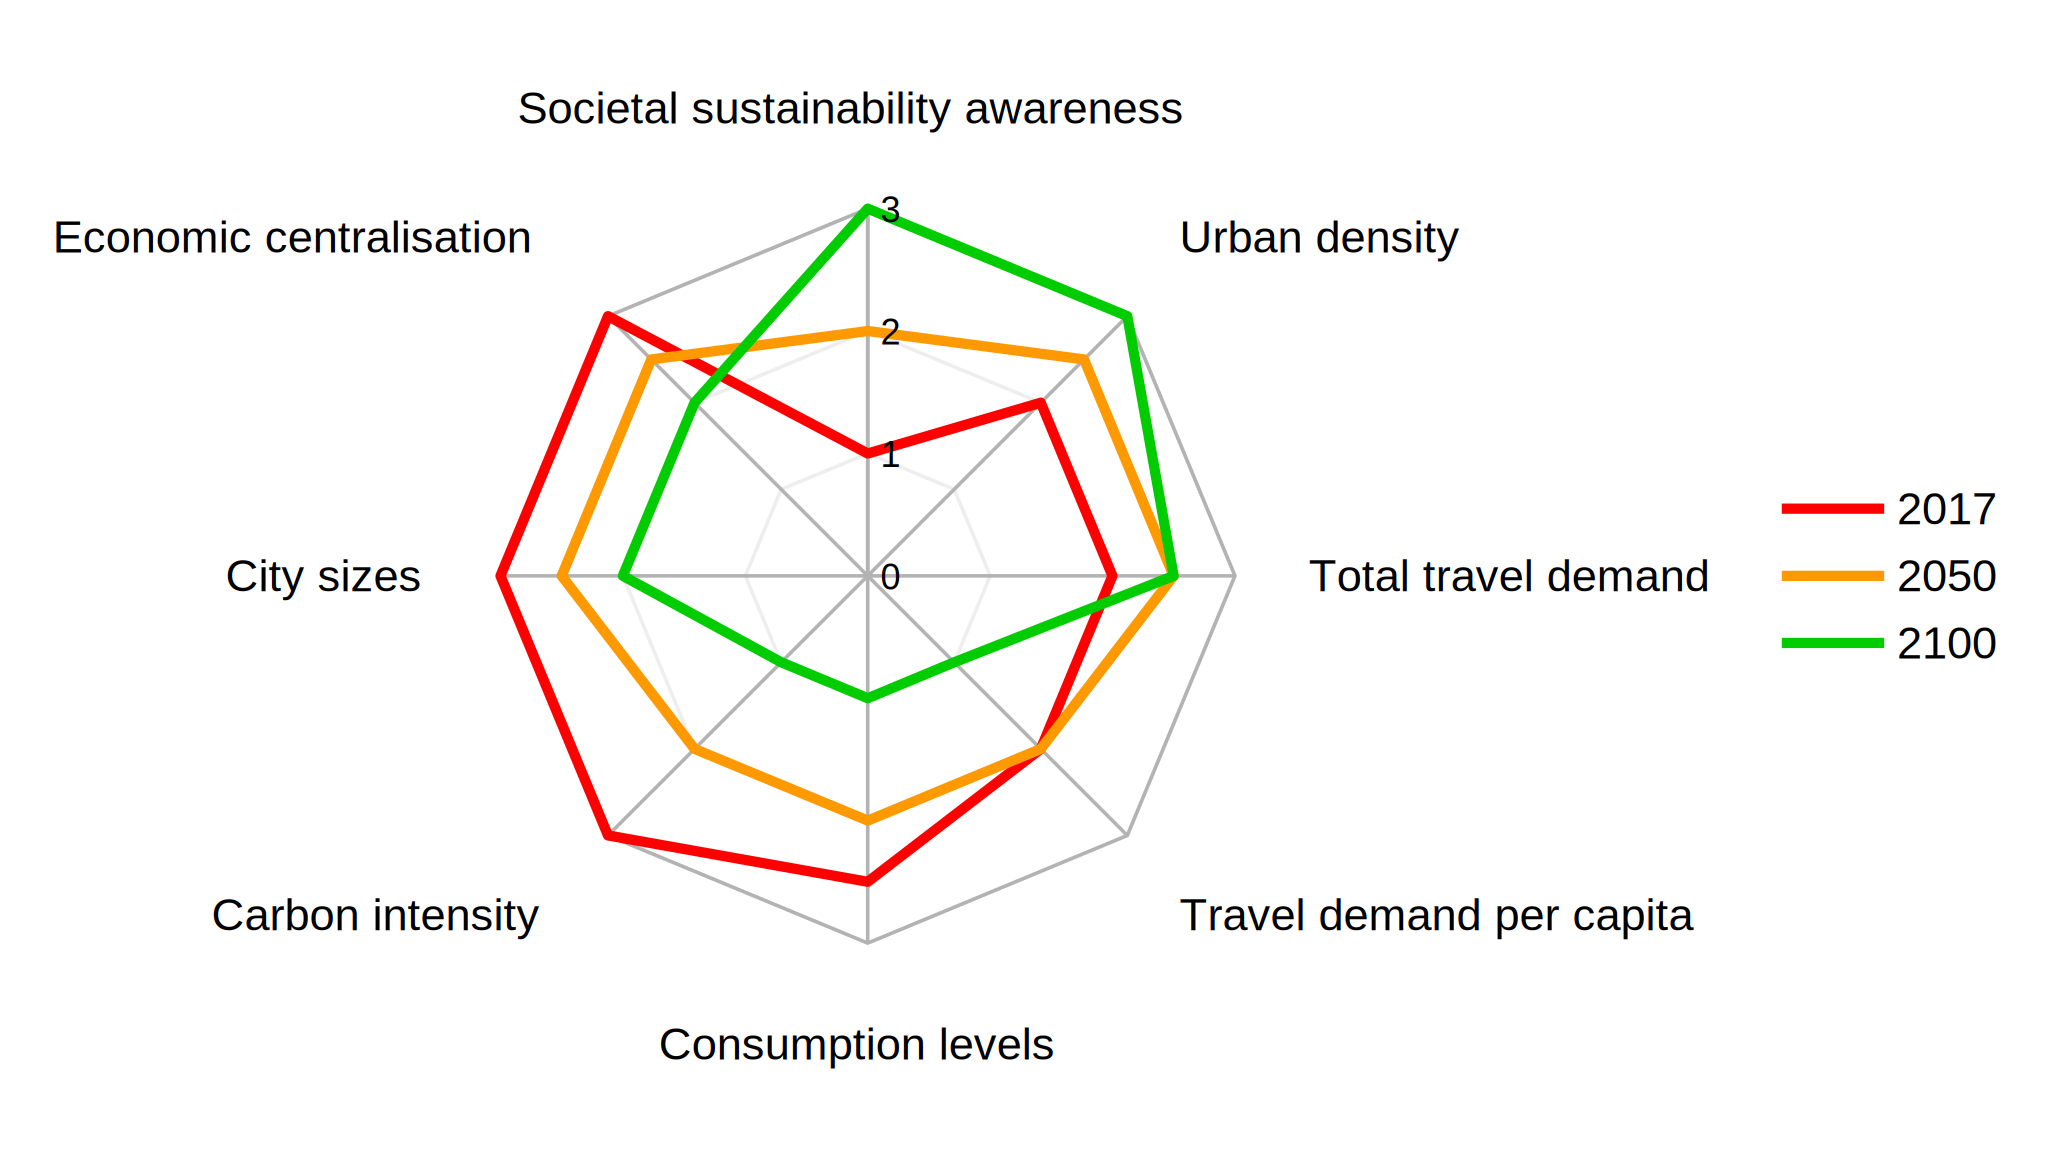
\includegraphics[width=0.8\textwidth]{figures/radar_development-scenario}
\caption[Shifts in development and land-use patterns in SSP1-MOB.]{Radar graph showing the shifts in development trends and land-use patterns found in SSP1 and SSP1-MOB for the years 2100, 2050 and 2017 (baseline). Values are given to the qualitative variables: 3 for high, 2 for medium and 1 for low.}
\label{fig:results:radar_development-scenario}
\end{figure}
%
\begin{figure}
		\centering
  \begin{subfigure}{0.8\textwidth}
    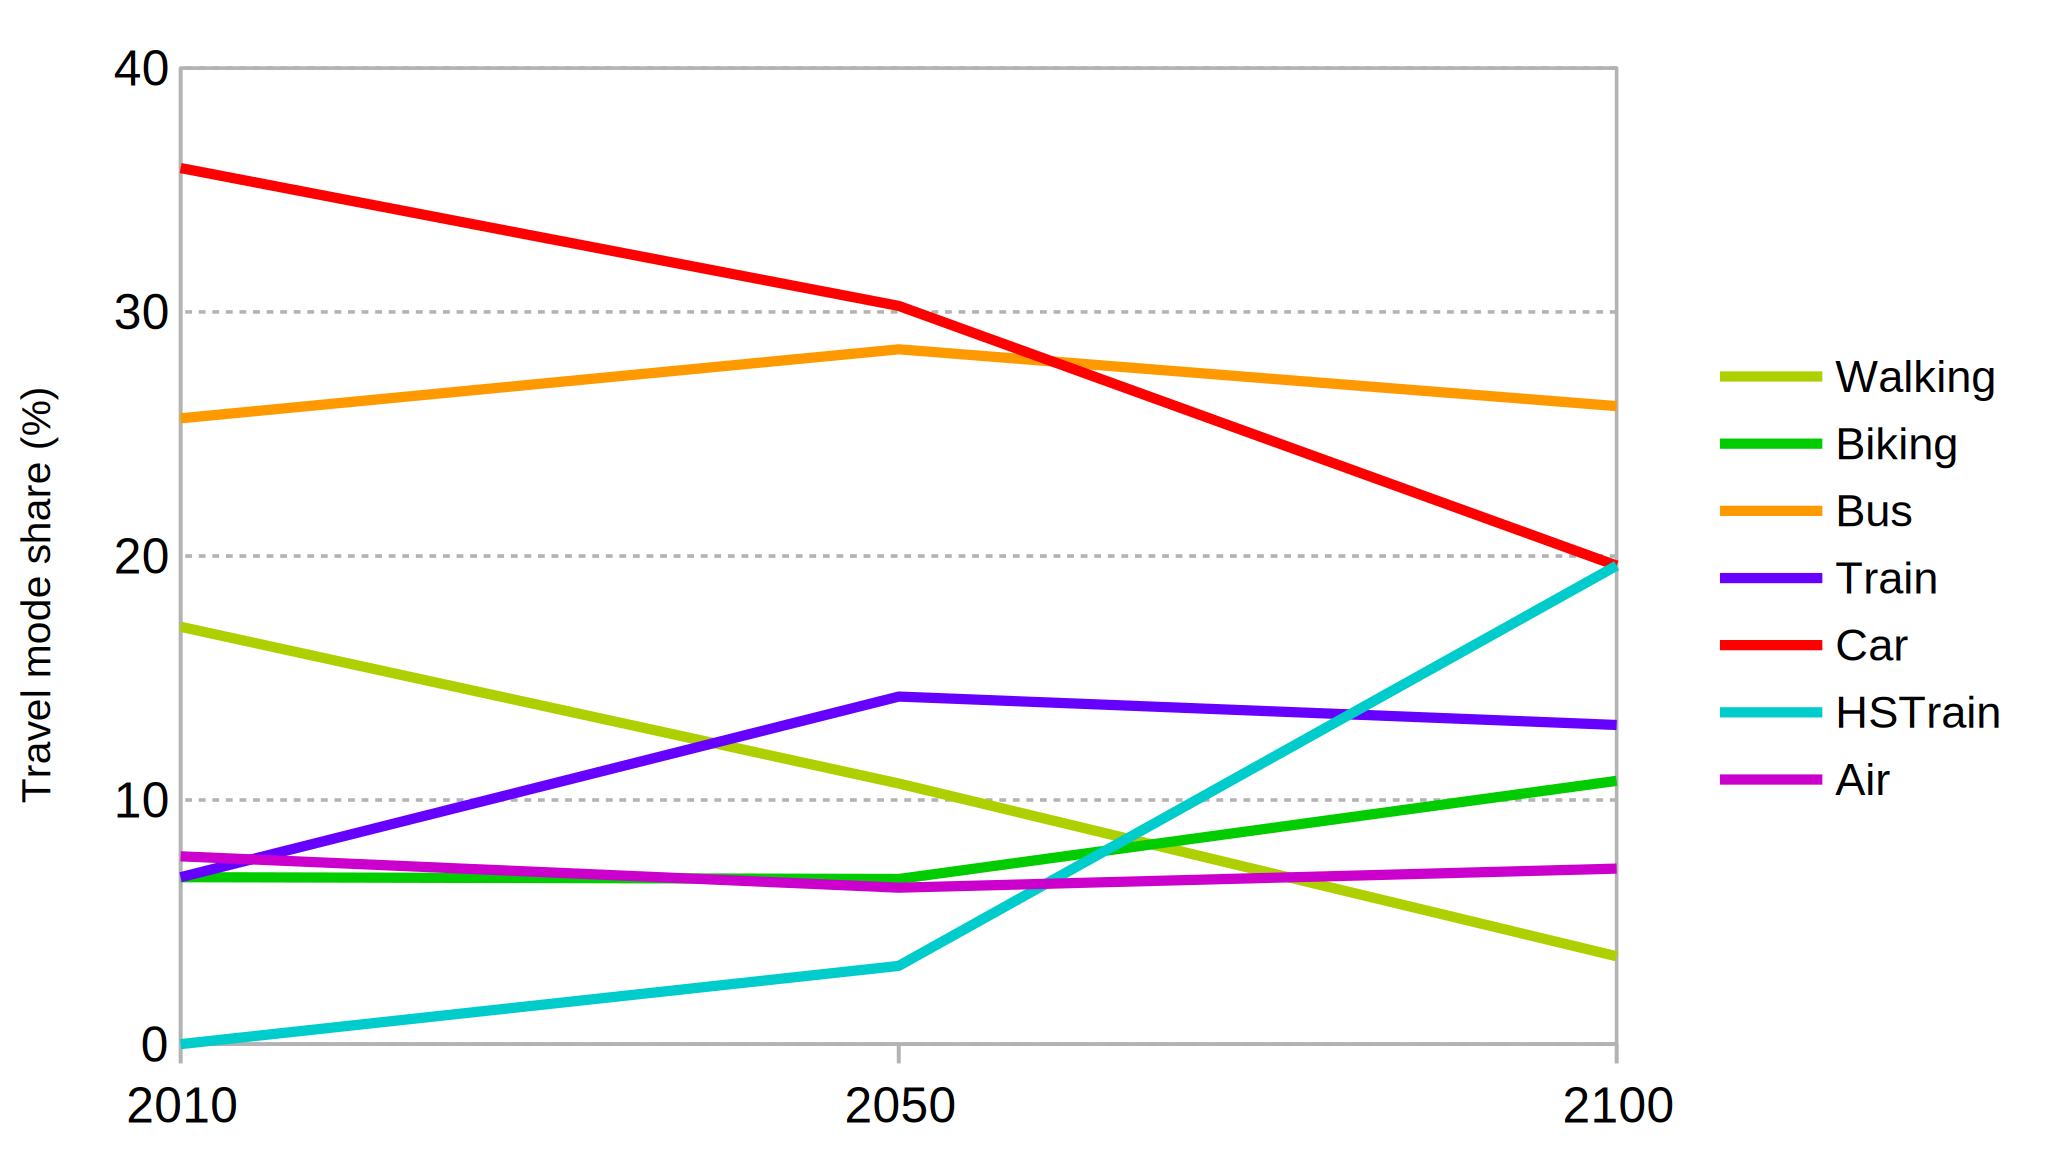
\includegraphics[width=\linewidth]{figures/line_travel-demand-shares.pdf}
    \caption{}
    \label{fig:results:line_travel-demand-shares}
  \end{subfigure}
  \begin{subfigure}{0.8\textwidth}
    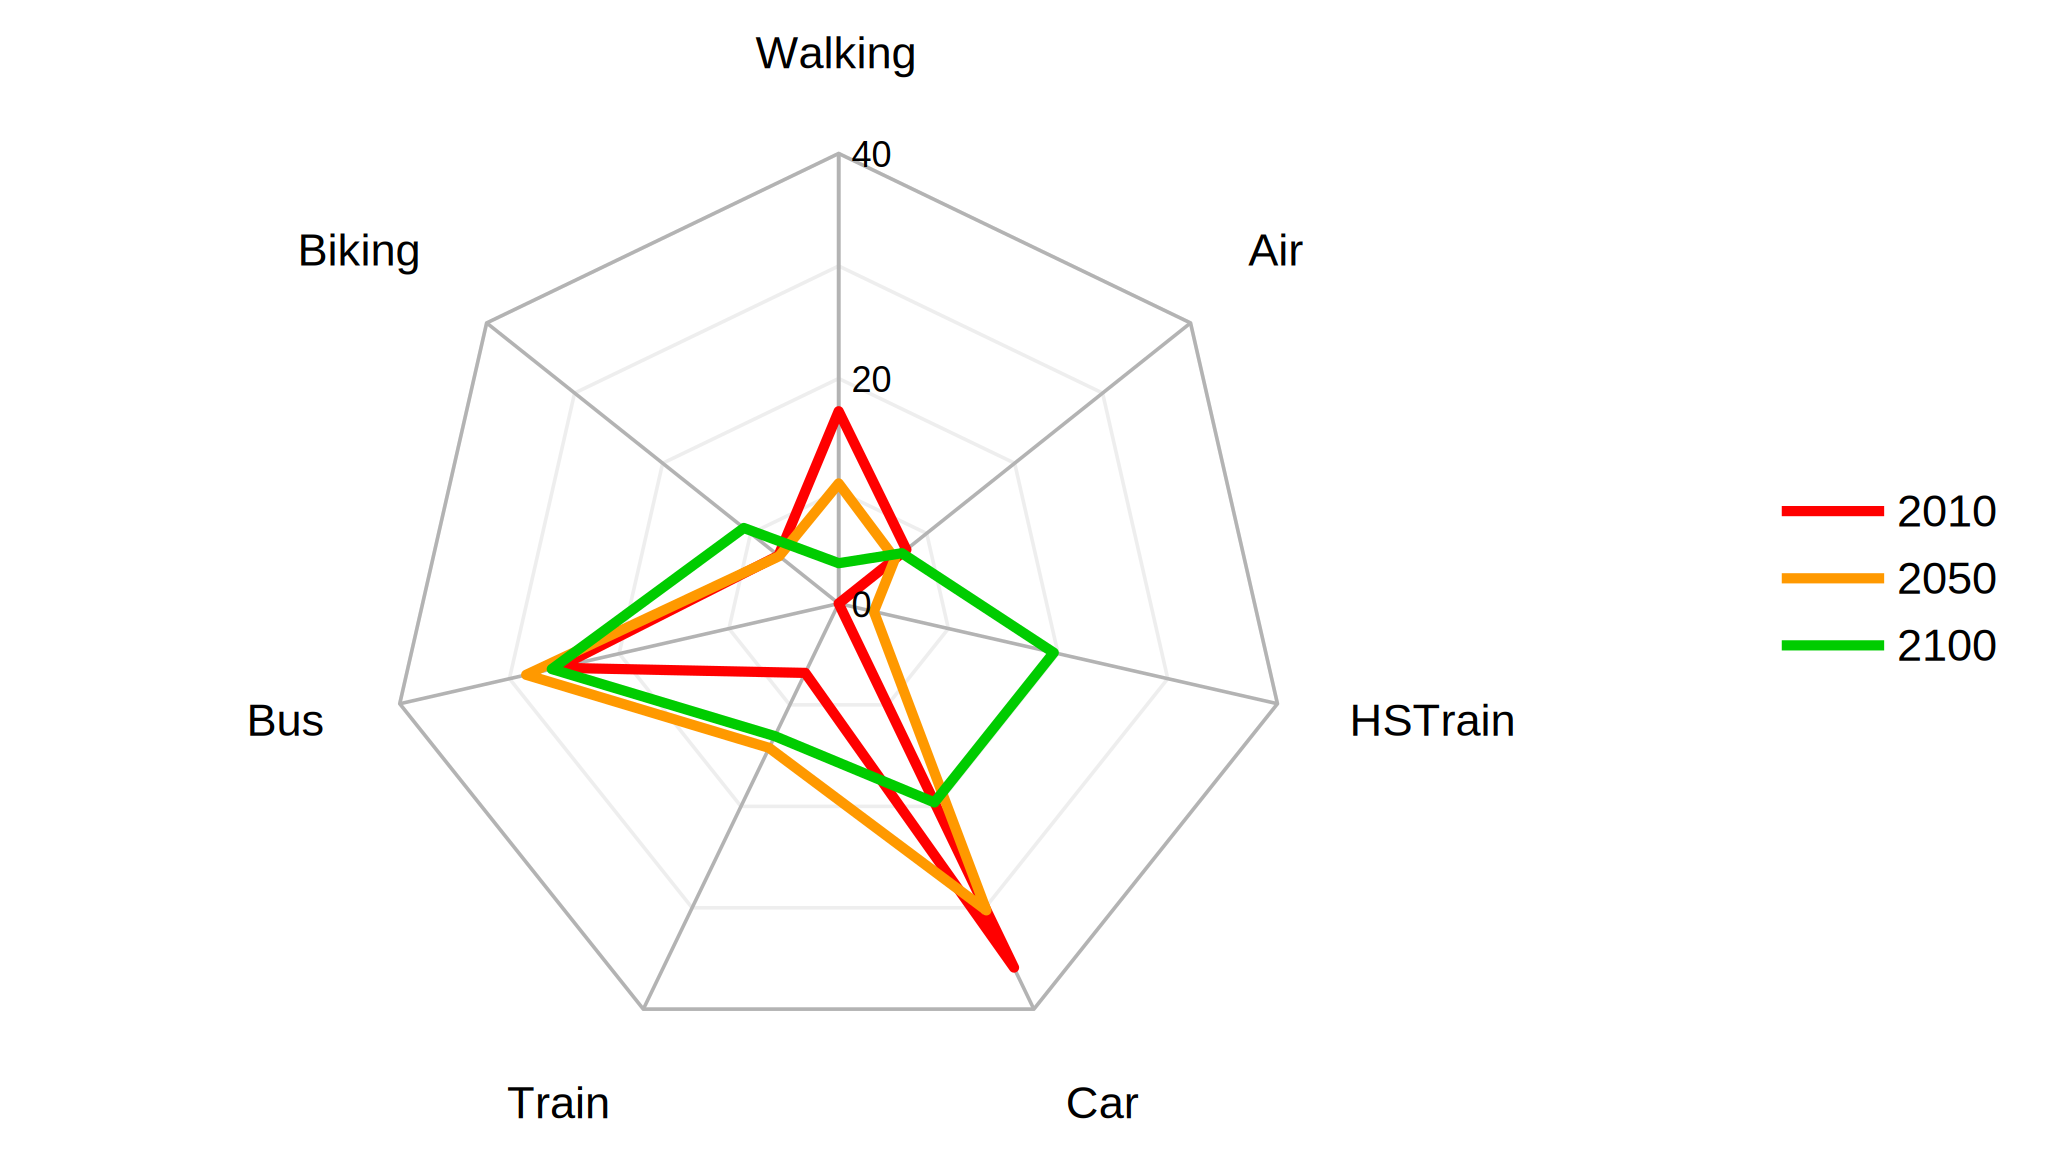
\includegraphics[width=\linewidth]{figures/radar_travel-demand-shares.pdf}
    \caption{}
    \label{fig:results:radar_travel-demand-shares}
  \end{subfigure}
  \caption[Evolution and comparison of travel demand shares in SSP1-MOB.]{Evolution (a) and comparison (b) of total travel demand per transport mode (shares), in percentages, across the SSP1-MOB futures and the 2017 baseline. Note: the demand shares are approximated from the figures provided by \textcite{vuuren2017_Energylanduse} in their quantitative appraisal of the SSP1 scenario.}
\end{figure}

\section[The AUTOLOCK model]{The AUTOLOCK model: understanding the feedback structures that drive the automobility regime}
\label{s:results:autolock-model}
This section is devoted to the investigation of the feedback structure that supports and shapes the system of automobility. \todonote{Perhaps this explanation of \emph{``why cars?''} could be in another chapter: methods? Introduction?}The choice of this particular transport mode is based on two arguments: first, the clear dominance of the automobile as the main mode of transport globally (travel demand) and second, the huge inertia, complexity and stability that the system has historically posed against threats to its dominance, e.g., the 1970s oil crisis, the ``dieselgate'' scandal\footnote{``Dieselgate'' refers to the Volkswagen emissions scandal that started in September 2015, when the U.S. Environmental Protection Agency reported that the German automotive industrial group had been faking emission control tests. This caused the \ce{NO_X} output to be lower in the certification tests than in real-world driving scenarios, thus being able to meet U.S. and European emission standards.} \parencite{guardian2017_Volkswagenrevealsrecord}, or even the 2008 global financial crisis. \fref{f:results:global-passenger-car-production} shows the global production of cars from 1961 to 2015, clearly depicting the effects of the financial crisis, whilst acknowledging that production has kept increasing nevertheless.
%
\begin{figure}[h]
\centering
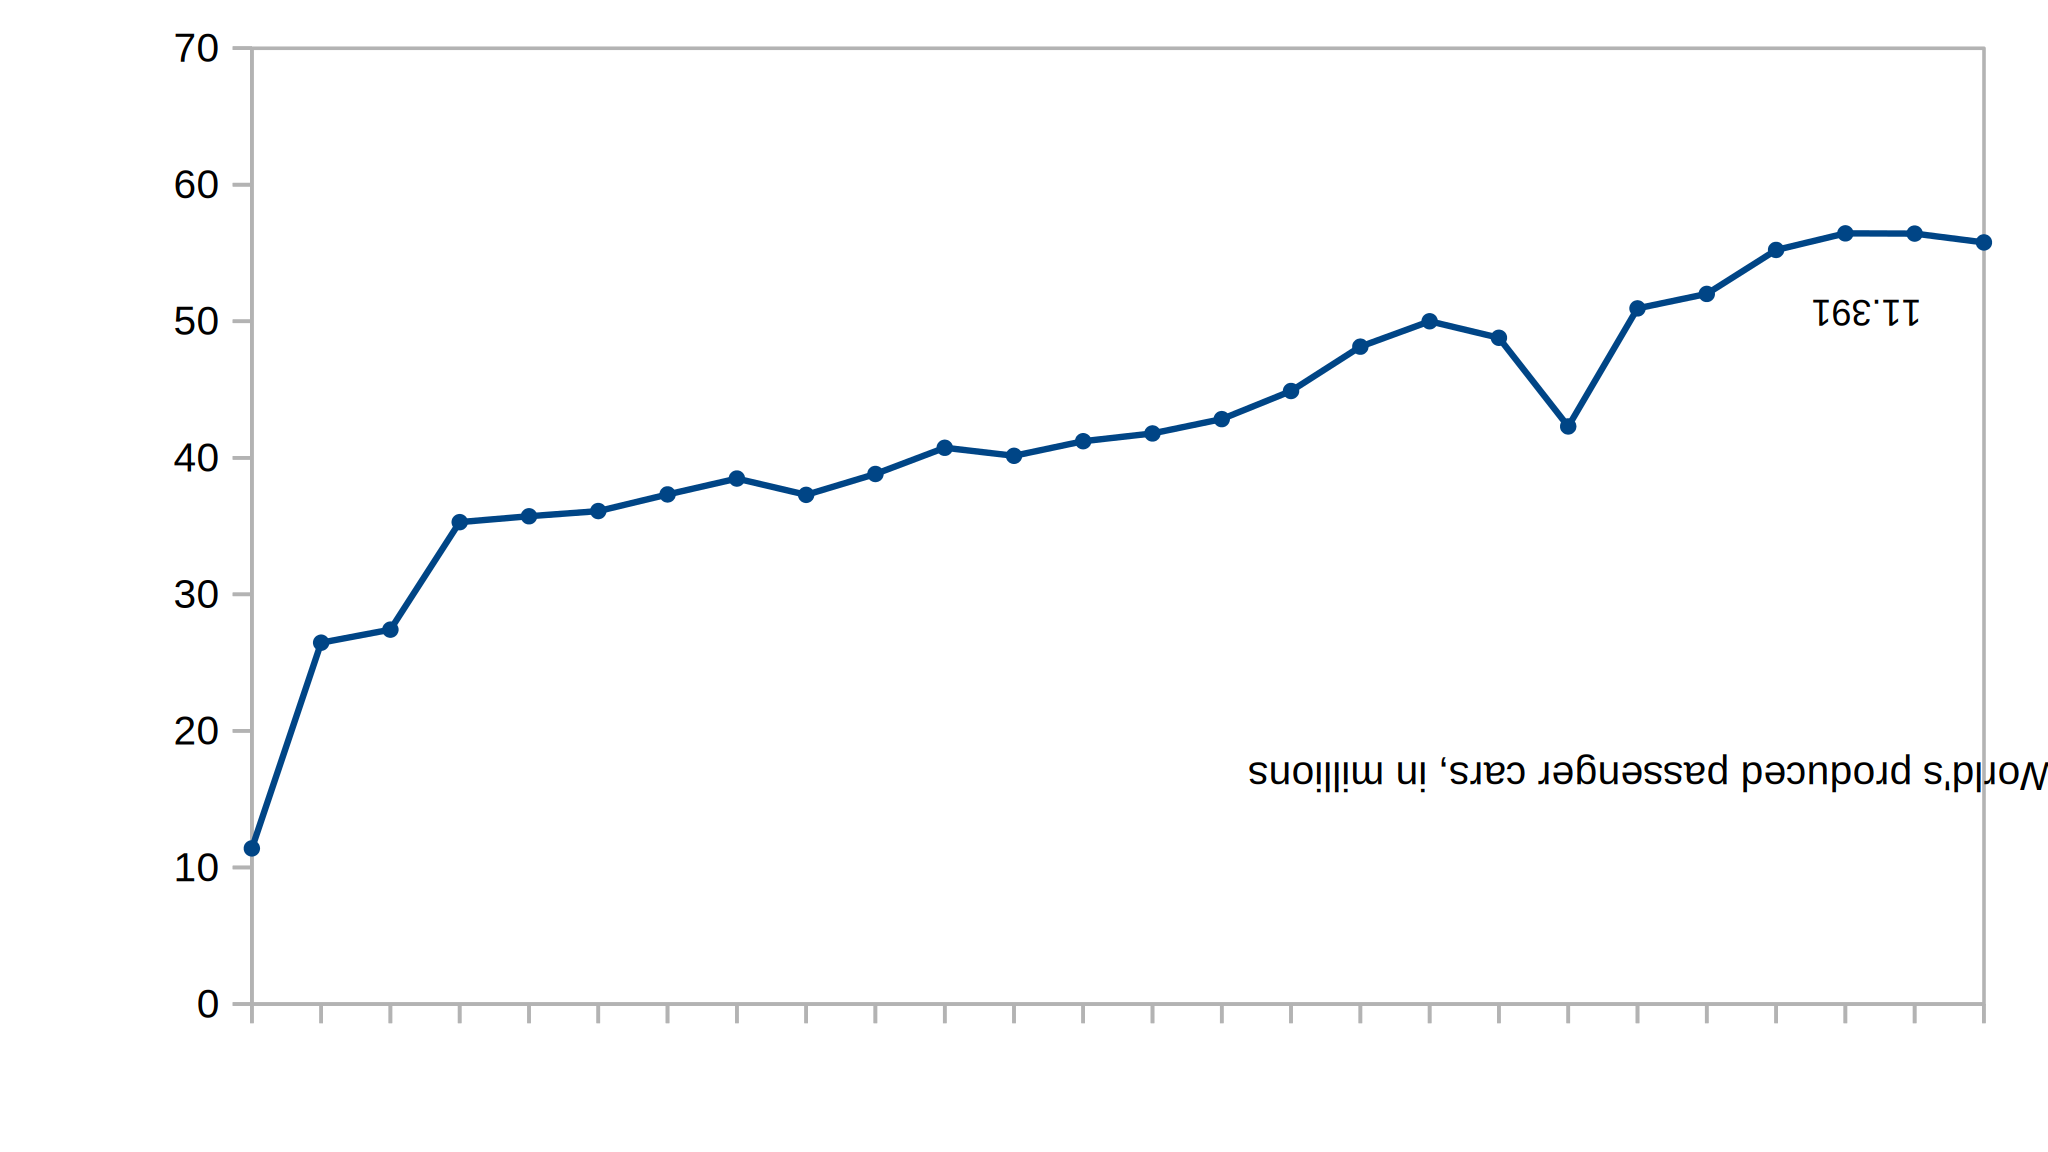
\includegraphics[width=0.8\textwidth]{figures/line_global-car-sales.pdf}
\label{f:results:global-passenger-car-production}
\caption[Global passenger cars production 1961-2015.]{Global passenger car production 1961-2015. Source: own figure; original data from \textcite{bts2017_Table123}.}
\end{figure}

As already mentioned in the \nameref{c:methods} chapter, the study of the feedback structures of the system, detailed in the following subsections, is carried out through a series of Causal Loop Diagrams (CLD). Because of the resilient nature of the automobility regime, the collection of CLDs that form the overview of the system is referred to as the AUTOLOCK model. \ssref{ss:results:cld_urban-planning} discusses the stability mechanisms of automobility from an urban planning (land use) perspective. The cultural basis and legitimacy apparatus of automobility is described in \ssref{ss:results:cld_cultural-feedbacks}. \ssref{ss:results:cld_public-transport-automobility} provides a (partial) explanation of how automobility displaces public transport and vice-versa. Finally, \todonote{Talk about PLPs}

\subsection{Urban planning and automobility}
\label{ss:results:cld_urban-planning}

\begin{figure}[h]
\centering
\fbox{\includegraphics[width=\textwidth]{figures/model/congestion-urban_1_core.pdf}}
\label{f:results:cld_congestion_1}
\caption[]{}
\end{figure}

\begin{figure}[h]
\centering
\fbox{\includegraphics[width=\textwidth]{figures/model/congestion-urban_2_dependency.pdf}}
\label{f:results:cld_congestion_2}
\caption[]{}
\end{figure}

\begin{landscape}
\begin{figure}
\centering
\fbox{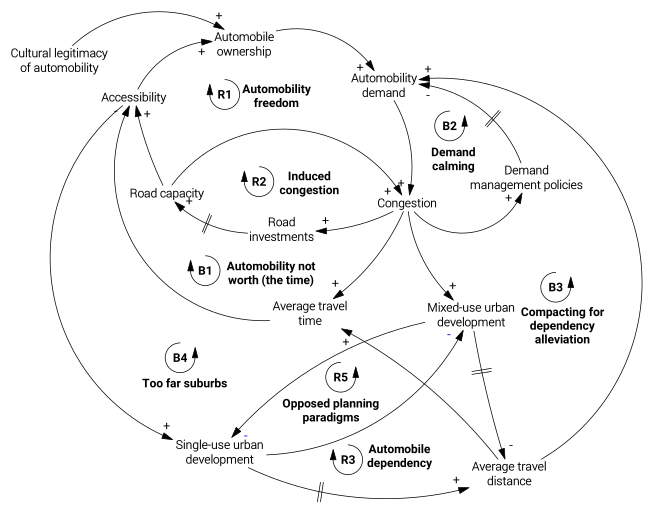
\includegraphics[width=\textwidth]{figures/model/congestion-urban_3_final.pdf}}
\label{f:results:cld_congestion_3}
\caption[]{}
\end{figure}
\end{landscape}

\subsection{Cultural feedbacks}
\label{ss:results:cld_cultural-feedbacks}

\begin{figure}[h]
\centering
\fbox{\includegraphics[width=\textwidth]{figures/model/cultural_1_core.pdf}}
\label{f:results:cld_culture_1}
\caption[]{}
\end{figure}

\begin{figure}[h]
\centering
\fbox{\includegraphics[width=\textwidth]{figures/model/cultural_2_class-relations.pdf}}
\label{f:results:cld_culture_2}
\caption[]{}
\end{figure}

\begin{landscape}
\begin{figure}
\centering
\fbox{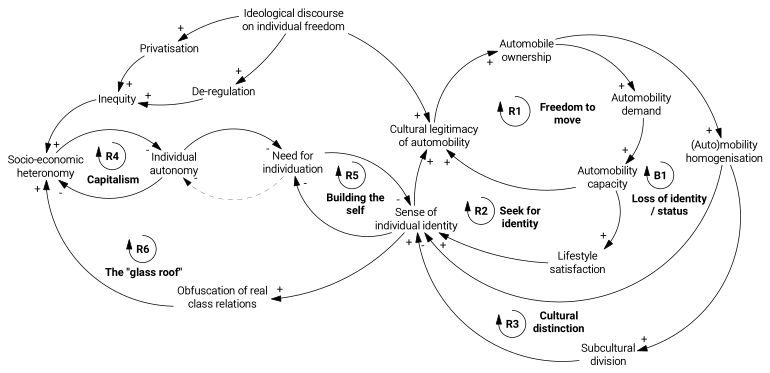
\includegraphics[width=\textwidth]{figures/model/cultural_3_final.pdf}}
\label{f:results:cld_culture_3}
\caption[]{}
\end{figure}
\end{landscape}

\subsection{Public transport vs. Automobility}
\label{ss:results:cld_public-transport-automobility}

\begin{figure}[h]
\centering
\fbox{\includegraphics[width=\textwidth]{figures/model/public-transport_1_core.pdf}}
\label{f:results:cld_pt_1}
\caption[]{}
\end{figure}

\begin{figure}[h]
\centering
\fbox{\includegraphics[width=\textwidth]{figures/model/public-transport_2_trust.pdf}}
\label{f:results:cld_pt_2}
\caption[]{}
\end{figure}

\begin{landscape}
\begin{figure}
\centering
\fbox{\includegraphics[width=\textwidth]{figures/model/public-transport_3_final.pdf}}
\label{f:results:cld_pt_3}
\caption[]{}
\end{figure}
\end{landscape}

\subsection{Identification of Policy Leverage Points}
\label{ss:results:cld_policy-leverage-points}

\section[Transition-oriented policy recommendations]{Transition-oriented policy recommendations for a future sustainable mobility}
\label{s:results:policy-recommendations}
% (Geels et al, 2012)
% The logic of the MLP suggests policy makers can follow two strategies
% to influence transitions:
%   i) Enhance pressure on regimes through economic instruments and regulation
%  ii) Stimulate the emergence and diffusion of niche innovations

\subsection{Niche level policies}
\label{ss:results:policies_niche}

\subsection{Regime level policies}
\label{ss:results:policies_regime}

\subsection{Landscape level policies}
\label{ss:results:policies_landscape}